\documentclass[]{article}
\usepackage{lmodern}
\usepackage{amssymb,amsmath}
\usepackage{ifxetex,ifluatex}
\usepackage{fixltx2e} % provides \textsubscript
\ifnum 0\ifxetex 1\fi\ifluatex 1\fi=0 % if pdftex
  \usepackage[T1]{fontenc}
  \usepackage[utf8]{inputenc}
\else % if luatex or xelatex
  \ifxetex
    \usepackage{mathspec}
  \else
    \usepackage{fontspec}
  \fi
  \defaultfontfeatures{Ligatures=TeX,Scale=MatchLowercase}
\fi
% use upquote if available, for straight quotes in verbatim environments
\IfFileExists{upquote.sty}{\usepackage{upquote}}{}
% use microtype if available
\IfFileExists{microtype.sty}{%
\usepackage[]{microtype}
\UseMicrotypeSet[protrusion]{basicmath} % disable protrusion for tt fonts
}{}
\PassOptionsToPackage{hyphens}{url} % url is loaded by hyperref
\usepackage[unicode=true]{hyperref}
\hypersetup{
            pdftitle={nlp\_tw},
            pdfauthor={haiyan yu},
            pdfborder={0 0 0},
            breaklinks=true}
\urlstyle{same}  % don't use monospace font for urls
\usepackage[margin=1in]{geometry}
\usepackage{color}
\usepackage{fancyvrb}
\newcommand{\VerbBar}{|}
\newcommand{\VERB}{\Verb[commandchars=\\\{\}]}
\DefineVerbatimEnvironment{Highlighting}{Verbatim}{commandchars=\\\{\}}
% Add ',fontsize=\small' for more characters per line
\usepackage{framed}
\definecolor{shadecolor}{RGB}{248,248,248}
\newenvironment{Shaded}{\begin{snugshade}}{\end{snugshade}}
\newcommand{\KeywordTok}[1]{\textcolor[rgb]{0.13,0.29,0.53}{\textbf{#1}}}
\newcommand{\DataTypeTok}[1]{\textcolor[rgb]{0.13,0.29,0.53}{#1}}
\newcommand{\DecValTok}[1]{\textcolor[rgb]{0.00,0.00,0.81}{#1}}
\newcommand{\BaseNTok}[1]{\textcolor[rgb]{0.00,0.00,0.81}{#1}}
\newcommand{\FloatTok}[1]{\textcolor[rgb]{0.00,0.00,0.81}{#1}}
\newcommand{\ConstantTok}[1]{\textcolor[rgb]{0.00,0.00,0.00}{#1}}
\newcommand{\CharTok}[1]{\textcolor[rgb]{0.31,0.60,0.02}{#1}}
\newcommand{\SpecialCharTok}[1]{\textcolor[rgb]{0.00,0.00,0.00}{#1}}
\newcommand{\StringTok}[1]{\textcolor[rgb]{0.31,0.60,0.02}{#1}}
\newcommand{\VerbatimStringTok}[1]{\textcolor[rgb]{0.31,0.60,0.02}{#1}}
\newcommand{\SpecialStringTok}[1]{\textcolor[rgb]{0.31,0.60,0.02}{#1}}
\newcommand{\ImportTok}[1]{#1}
\newcommand{\CommentTok}[1]{\textcolor[rgb]{0.56,0.35,0.01}{\textit{#1}}}
\newcommand{\DocumentationTok}[1]{\textcolor[rgb]{0.56,0.35,0.01}{\textbf{\textit{#1}}}}
\newcommand{\AnnotationTok}[1]{\textcolor[rgb]{0.56,0.35,0.01}{\textbf{\textit{#1}}}}
\newcommand{\CommentVarTok}[1]{\textcolor[rgb]{0.56,0.35,0.01}{\textbf{\textit{#1}}}}
\newcommand{\OtherTok}[1]{\textcolor[rgb]{0.56,0.35,0.01}{#1}}
\newcommand{\FunctionTok}[1]{\textcolor[rgb]{0.00,0.00,0.00}{#1}}
\newcommand{\VariableTok}[1]{\textcolor[rgb]{0.00,0.00,0.00}{#1}}
\newcommand{\ControlFlowTok}[1]{\textcolor[rgb]{0.13,0.29,0.53}{\textbf{#1}}}
\newcommand{\OperatorTok}[1]{\textcolor[rgb]{0.81,0.36,0.00}{\textbf{#1}}}
\newcommand{\BuiltInTok}[1]{#1}
\newcommand{\ExtensionTok}[1]{#1}
\newcommand{\PreprocessorTok}[1]{\textcolor[rgb]{0.56,0.35,0.01}{\textit{#1}}}
\newcommand{\AttributeTok}[1]{\textcolor[rgb]{0.77,0.63,0.00}{#1}}
\newcommand{\RegionMarkerTok}[1]{#1}
\newcommand{\InformationTok}[1]{\textcolor[rgb]{0.56,0.35,0.01}{\textbf{\textit{#1}}}}
\newcommand{\WarningTok}[1]{\textcolor[rgb]{0.56,0.35,0.01}{\textbf{\textit{#1}}}}
\newcommand{\AlertTok}[1]{\textcolor[rgb]{0.94,0.16,0.16}{#1}}
\newcommand{\ErrorTok}[1]{\textcolor[rgb]{0.64,0.00,0.00}{\textbf{#1}}}
\newcommand{\NormalTok}[1]{#1}
\usepackage{graphicx,grffile}
\makeatletter
\def\maxwidth{\ifdim\Gin@nat@width>\linewidth\linewidth\else\Gin@nat@width\fi}
\def\maxheight{\ifdim\Gin@nat@height>\textheight\textheight\else\Gin@nat@height\fi}
\makeatother
% Scale images if necessary, so that they will not overflow the page
% margins by default, and it is still possible to overwrite the defaults
% using explicit options in \includegraphics[width, height, ...]{}
\setkeys{Gin}{width=\maxwidth,height=\maxheight,keepaspectratio}
\IfFileExists{parskip.sty}{%
\usepackage{parskip}
}{% else
\setlength{\parindent}{0pt}
\setlength{\parskip}{6pt plus 2pt minus 1pt}
}
\setlength{\emergencystretch}{3em}  % prevent overfull lines
\providecommand{\tightlist}{%
  \setlength{\itemsep}{0pt}\setlength{\parskip}{0pt}}
\setcounter{secnumdepth}{0}
% Redefines (sub)paragraphs to behave more like sections
\ifx\paragraph\undefined\else
\let\oldparagraph\paragraph
\renewcommand{\paragraph}[1]{\oldparagraph{#1}\mbox{}}
\fi
\ifx\subparagraph\undefined\else
\let\oldsubparagraph\subparagraph
\renewcommand{\subparagraph}[1]{\oldsubparagraph{#1}\mbox{}}
\fi

% set default figure placement to htbp
\makeatletter
\def\fps@figure{htbp}
\makeatother


\title{nlp\_tw}
\author{haiyan yu}
\date{2/21/2020}

\begin{document}
\maketitle

\begin{Shaded}
\begin{Highlighting}[]
\KeywordTok{library}\NormalTok{(tm)}
\end{Highlighting}
\end{Shaded}

\begin{verbatim}
## Loading required package: NLP
\end{verbatim}

\begin{Shaded}
\begin{Highlighting}[]
\KeywordTok{library}\NormalTok{(NLP)}
\KeywordTok{library}\NormalTok{(jiebaR)}
\end{Highlighting}
\end{Shaded}

\begin{verbatim}
## Loading required package: jiebaRD
\end{verbatim}

\begin{Shaded}
\begin{Highlighting}[]
\KeywordTok{library}\NormalTok{(plyr)}
\KeywordTok{library}\NormalTok{(readxl)}
\KeywordTok{library}\NormalTok{(HMM)}
\CommentTok{#library(xlsx)}
\KeywordTok{library}\NormalTok{(Rwordseg)}
\end{Highlighting}
\end{Shaded}

\begin{verbatim}
## Loading required package: tmcn
\end{verbatim}

\begin{verbatim}
## # tmcn Version: 0.2-13
\end{verbatim}

\begin{verbatim}
## HMM model has been loaded.
\end{verbatim}

\begin{verbatim}
## # 
## The defalut analyzer is 'hmm' implemented by native R codes, which is still in development.
\end{verbatim}

\begin{verbatim}
## If you want to improve the performance you can choose:
\end{verbatim}

\begin{verbatim}
##   - "jiebaR", a popular segmentation module, by running "setAnalyzer('jiebaR')".
\end{verbatim}

\begin{verbatim}
##   - "coreNLP", a R wrappers around Stanford CoreNLP, by running "setAnalyzer('coreNLP')".
\end{verbatim}

\begin{verbatim}
##   - "fmm", the easiest way of using forward maximum matching algorithm, by running "setAnalyzer('fmm')".
\end{verbatim}

\begin{Shaded}
\begin{Highlighting}[]
\KeywordTok{library}\NormalTok{(dplyr)}
\end{Highlighting}
\end{Shaded}

\begin{verbatim}
## 
## Attaching package: 'dplyr'
\end{verbatim}

\begin{verbatim}
## The following objects are masked from 'package:plyr':
## 
##     arrange, count, desc, failwith, id, mutate, rename, summarise,
##     summarize
\end{verbatim}

\begin{verbatim}
## The following objects are masked from 'package:stats':
## 
##     filter, lag
\end{verbatim}

\begin{verbatim}
## The following objects are masked from 'package:base':
## 
##     intersect, setdiff, setequal, union
\end{verbatim}

\begin{Shaded}
\begin{Highlighting}[]
\KeywordTok{library}\NormalTok{(tidytext)}
\KeywordTok{library}\NormalTok{(ggplot2)}
\end{Highlighting}
\end{Shaded}

\begin{verbatim}
## 
## Attaching package: 'ggplot2'
\end{verbatim}

\begin{verbatim}
## The following object is masked from 'package:NLP':
## 
##     annotate
\end{verbatim}

\begin{Shaded}
\begin{Highlighting}[]
\KeywordTok{library}\NormalTok{(stringr)}
\KeywordTok{library}\NormalTok{(igraph)}
\end{Highlighting}
\end{Shaded}

\begin{verbatim}
## 
## Attaching package: 'igraph'
\end{verbatim}

\begin{verbatim}
## The following objects are masked from 'package:dplyr':
## 
##     as_data_frame, groups, union
\end{verbatim}

\begin{verbatim}
## The following objects are masked from 'package:stats':
## 
##     decompose, spectrum
\end{verbatim}

\begin{verbatim}
## The following object is masked from 'package:base':
## 
##     union
\end{verbatim}

\begin{Shaded}
\begin{Highlighting}[]
\KeywordTok{library}\NormalTok{(ggraph)}
\KeywordTok{library}\NormalTok{(tidyr)}
\end{Highlighting}
\end{Shaded}

\begin{verbatim}
## 
## Attaching package: 'tidyr'
\end{verbatim}

\begin{verbatim}
## The following object is masked from 'package:igraph':
## 
##     crossing
\end{verbatim}

\section{二、计算词频表}\label{ux4e8cux8ba1ux7b97ux8bcdux9891ux8868}

\begin{Shaded}
\begin{Highlighting}[]
\CommentTok{#加载文件}
\NormalTok{file_}\DecValTok{1}\NormalTok{<-}\KeywordTok{read.csv}\NormalTok{(}\StringTok{"~/Downloads/Rpkg/nlph/data/merge.csv"}\NormalTok{,}
                 \DataTypeTok{header =} \OtherTok{TRUE}\NormalTok{, }\DataTypeTok{sep =} \StringTok{","}\NormalTok{, }\DataTypeTok{quote=}\StringTok{"}\CharTok{\textbackslash{}"}\StringTok{"}\NormalTok{, }\DataTypeTok{encoding =} \StringTok{"UTF-8"}\NormalTok{,}
                 \DataTypeTok{stringsAsFactors =} \OtherTok{TRUE}\NormalTok{)}
\CommentTok{#将text列数据转成character类型}
\NormalTok{file_}\DecValTok{1}\OperatorTok{$}\NormalTok{text <-}\StringTok{ }\KeywordTok{as.character}\NormalTok{(file_}\DecValTok{1}\OperatorTok{$}\NormalTok{text)}
\NormalTok{txtFile<-file_}\DecValTok{1}\OperatorTok{$}\NormalTok{text}
\NormalTok{engin1<-}\KeywordTok{worker}\NormalTok{()}
\CommentTok{#对文本进行分词处理}
\NormalTok{segWords<-}\KeywordTok{segment}\NormalTok{(txtFile,engin1)}
\CommentTok{#停止词的处理}
\NormalTok{mystopwords<-}\StringTok{ }\KeywordTok{readLines}\NormalTok{(}\StringTok{'~/Downloads/Rpkg/nlph/data/en-stopword.txt'}\NormalTok{)}
\NormalTok{segWords<-}\KeywordTok{removeWords}\NormalTok{(segWords,mystopwords)}
\CommentTok{#去除数字和标点符号}
\NormalTok{segWords<-}\KeywordTok{gsub}\NormalTok{(}\StringTok{'}\CharTok{\textbackslash{}\textbackslash{}}\StringTok{d|}\CharTok{\textbackslash{}\textbackslash{}}\StringTok{.|,|}\CharTok{\textbackslash{}\textbackslash{}}\StringTok{!|:|;|}\CharTok{\textbackslash{}\textbackslash{}}\StringTok{?'}\NormalTok{,}\StringTok{""}\NormalTok{,segWords)}
\CommentTok{#到此为止,清洗完成}
\NormalTok{sre<-}\KeywordTok{sort}\NormalTok{(}\KeywordTok{table}\NormalTok{(segWords),}\DataTypeTok{decreasing =} \OtherTok{TRUE}\NormalTok{)}
\CommentTok{#输出组合后的文件wordFreq.csv到文件夹}
\CommentTok{#write.csv(sre,file = "~/Downloads/Rpkg/nlph/data/wordFreq2.csv",row.names=F)}

\NormalTok{sre.df<-}\KeywordTok{data.frame}\NormalTok{(sre)}
\KeywordTok{head}\NormalTok{(sre.df[sre.df}\OperatorTok{$}\NormalTok{Freq}\OperatorTok{>}\DecValTok{500}\NormalTok{,])}
\end{Highlighting}
\end{Shaded}

\begin{verbatim}
##      segWords  Freq
## 1             93186
## 2 coronavirus  7373
## 3       China  5075
## 4    outbreak  2784
## 5       Wuhan  2261
## 6      people  1036
\end{verbatim}

\begin{Shaded}
\begin{Highlighting}[]
\NormalTok{sredf.df <-}\StringTok{ }\KeywordTok{data.frame}\NormalTok{(}\DataTypeTok{stringsAsFactors=}\OtherTok{FALSE}\NormalTok{,}
                 \DataTypeTok{word =}\NormalTok{ sre.df}\OperatorTok{$}\NormalTok{segWords,}
                 \DataTypeTok{freq =}\NormalTok{ sre.df}\OperatorTok{$}\NormalTok{Freq)}
\CommentTok{# "1" blank}
\NormalTok{sredf.df<-sredf.df[}\DecValTok{2}\OperatorTok{:}\DecValTok{30}\NormalTok{,]}
\KeywordTok{library}\NormalTok{(ggplot2)}

\KeywordTok{ggplot}\NormalTok{(sredf.df, }\KeywordTok{aes}\NormalTok{(}\DataTypeTok{x =} \KeywordTok{reorder}\NormalTok{(word, freq), }\DataTypeTok{y =}\NormalTok{ freq)) }\OperatorTok{+}
\StringTok{    }\KeywordTok{geom_col}\NormalTok{() }\OperatorTok{+}
\StringTok{    }\KeywordTok{labs}\NormalTok{(}\DataTypeTok{title=}\StringTok{"Twitter "}\NormalTok{,}
         \DataTypeTok{x =} \OtherTok{NULL}\NormalTok{,}
         \DataTypeTok{y =} \StringTok{"Frequency"}\NormalTok{) }\OperatorTok{+}
\StringTok{    }\KeywordTok{coord_flip}\NormalTok{()}
\end{Highlighting}
\end{Shaded}

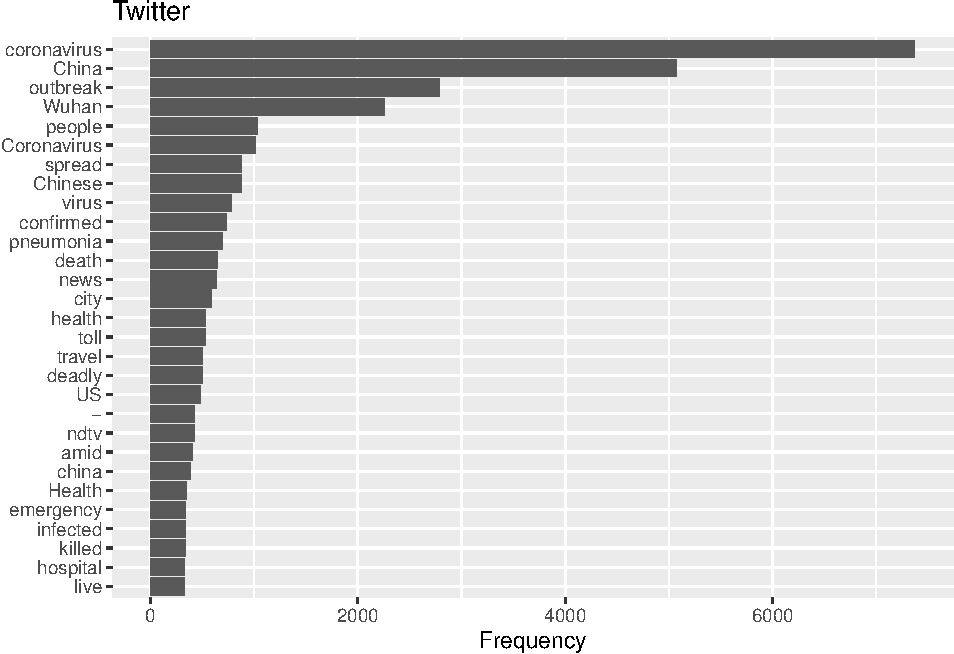
\includegraphics{nlp_tw_files/figure-latex/unnamed-chunk-2-1.pdf}

\section{三、知识网络图}\label{ux4e09ux77e5ux8bc6ux7f51ux7edcux56fe}

\begin{Shaded}
\begin{Highlighting}[]
\CommentTok{#注:若需要计算其他文件网络图,只需改变read.csv()函数中的文件路径和文件中需要提取的列}
\CommentTok{#加载文件}
\NormalTok{file_}\DecValTok{1}\NormalTok{<-}\KeywordTok{read.csv}\NormalTok{(}\StringTok{"~/Downloads/Rpkg/nlph/data/merge.csv"}\NormalTok{,}
                 \DataTypeTok{header =} \OtherTok{TRUE}\NormalTok{, }\DataTypeTok{sep =} \StringTok{","}\NormalTok{, }\DataTypeTok{quote=}\StringTok{"}\CharTok{\textbackslash{}"}\StringTok{"}\NormalTok{, }\DataTypeTok{encoding =} \StringTok{"UTF-8"}\NormalTok{,}
                 \DataTypeTok{stringsAsFactors =} \OtherTok{TRUE}\NormalTok{)}
\CommentTok{#读取text列文本}
\NormalTok{fi_}\DecValTok{1}\NormalTok{<-file_}\DecValTok{1}\NormalTok{[}\DecValTok{7}\NormalTok{]}
\NormalTok{austen_bigrams <-}\StringTok{ }\NormalTok{fi_}\DecValTok{1} \OperatorTok
\StringTok{  }\KeywordTok{unnest_tokens}\NormalTok{(bigram, text, }\DataTypeTok{token =} \StringTok{"ngrams"}\NormalTok{, }\DataTypeTok{n =} \DecValTok{2}\NormalTok{)}\OperatorTok
\StringTok{  }\KeywordTok{separate}\NormalTok{(bigram, }\KeywordTok{c}\NormalTok{(}\StringTok{"word1"}\NormalTok{, }\StringTok{"word2"}\NormalTok{), }\DataTypeTok{sep =} \StringTok{" "}\NormalTok{) }\OperatorTok
\StringTok{  }\KeywordTok{filter}\NormalTok{(}\OperatorTok{!}\NormalTok{word1 }\OperatorTok\StringTok{ }\NormalTok{stop_words}\OperatorTok{$}\NormalTok{word,}
         \OperatorTok{!}\NormalTok{word2 }\OperatorTok\StringTok{ }\NormalTok{stop_words}\OperatorTok{$}\NormalTok{word,}
         \OperatorTok{!}\KeywordTok{str_detect}\NormalTok{(word1,}\StringTok{'https'}\NormalTok{),}\OperatorTok{!}\KeywordTok{str_detect}\NormalTok{(word1,}\StringTok{'http'}\NormalTok{),}\OperatorTok{!}\KeywordTok{str_detect}\NormalTok{(word1,}\StringTok{'www.ndtv.com'}\NormalTok{),}
         \OperatorTok{!}\KeywordTok{str_detect}\NormalTok{(word2,}\StringTok{'https'}\NormalTok{),}\OperatorTok{!}\KeywordTok{str_detect}\NormalTok{(word2,}\StringTok{'http'}\NormalTok{)}
\NormalTok{  ) }\OperatorTok
\CommentTok{#  count(word1, word2)}
\StringTok{  }\KeywordTok{count}\NormalTok{(word1, word2, }\DataTypeTok{sort =} \OtherTok{TRUE}\NormalTok{)}
\CommentTok{#输出组合后的文件n-gram.csv到文件夹}
\KeywordTok{write.csv}\NormalTok{(austen_bigrams,}
          \DataTypeTok{file =} \StringTok{"~/Downloads/Rpkg/nlph/data/n-gram-new.csv"}\NormalTok{,}\DataTypeTok{row.names=}\NormalTok{F)}


\CommentTok{#画图}
\KeywordTok{set.seed}\NormalTok{(}\DecValTok{2016}\NormalTok{)}
\NormalTok{austen_bigrams<-}\KeywordTok{read.csv}\NormalTok{(}\DataTypeTok{file =} \StringTok{"~/Downloads//Rpkg/nlph/data/n-gram-new.csv"}\NormalTok{)}
\NormalTok{austen_bigrams_p<-austen_bigrams[austen_bigrams}\OperatorTok{$}\NormalTok{n}\OperatorTok{>}\DecValTok{100}\NormalTok{,]}
\KeywordTok{head}\NormalTok{(austen_bigrams)}
\end{Highlighting}
\end{Shaded}

\begin{verbatim}
##         word1       word2    n
## 1 coronavirus    outbreak 1817
## 2       wuhan coronavirus  698
## 3       death        toll  523
## 4       china coronavirus  421
## 5      deadly coronavirus  277
## 6       world        news  235
\end{verbatim}

\begin{Shaded}
\begin{Highlighting}[]
\NormalTok{a <-}\StringTok{ }\NormalTok{grid}\OperatorTok{::}\KeywordTok{arrow}\NormalTok{(}\DataTypeTok{type =} \StringTok{"closed"}\NormalTok{, }\DataTypeTok{length =} \KeywordTok{unit}\NormalTok{(.}\DecValTok{15}\NormalTok{, }\StringTok{"inches"}\NormalTok{))}

\KeywordTok{ggraph}\NormalTok{(austen_bigrams_p, }\DataTypeTok{layout =} \StringTok{"fr"}\NormalTok{) }\OperatorTok{+}
\StringTok{  }\KeywordTok{geom_edge_link}\NormalTok{(}\KeywordTok{aes}\NormalTok{(}\DataTypeTok{edge_alpha =}\NormalTok{ n), }\DataTypeTok{show.legend =} \OtherTok{FALSE}\NormalTok{,}
                 \DataTypeTok{arrow =}\NormalTok{ a, }\DataTypeTok{end_cap =} \KeywordTok{circle}\NormalTok{(.}\DecValTok{07}\NormalTok{, }\StringTok{'inches'}\NormalTok{)) }\OperatorTok{+}
\StringTok{  }\KeywordTok{geom_node_point}\NormalTok{(}\DataTypeTok{color =} \StringTok{"lightblue"}\NormalTok{, }\DataTypeTok{size =} \DecValTok{5}\NormalTok{) }\OperatorTok{+}
\StringTok{  }\KeywordTok{geom_node_text}\NormalTok{(}\KeywordTok{aes}\NormalTok{(}\DataTypeTok{label =}\NormalTok{ name), }\DataTypeTok{vjust =} \FloatTok{0.5}\NormalTok{, }\DataTypeTok{hjust =} \FloatTok{0.5}\NormalTok{) }\OperatorTok{+}
\StringTok{  }\KeywordTok{theme_void}\NormalTok{()}
\end{Highlighting}
\end{Shaded}

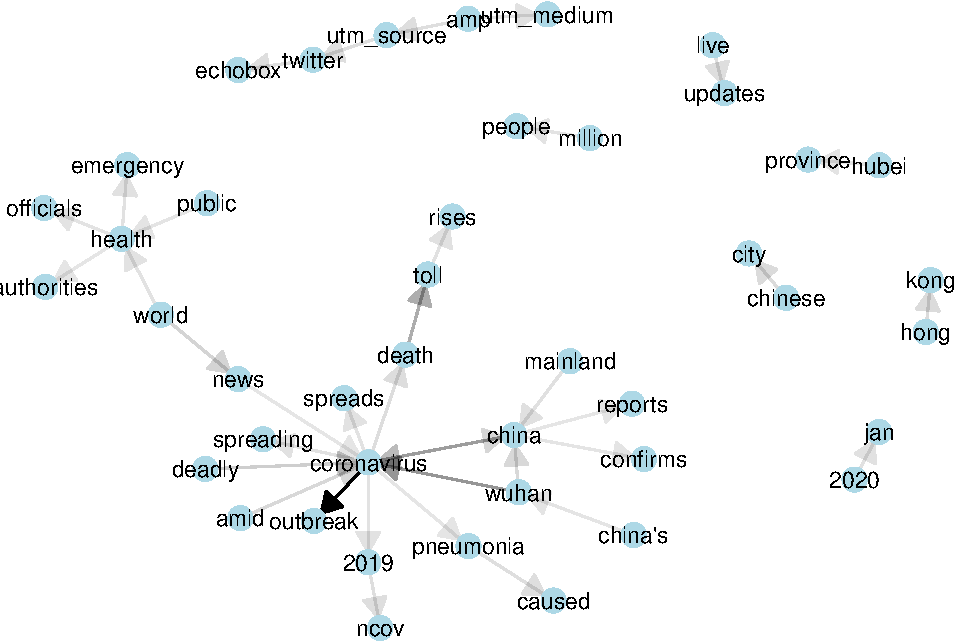
\includegraphics{nlp_tw_files/figure-latex/unnamed-chunk-3-1.pdf}

\section{情感:量化}\label{ux60c5ux611fux91cfux5316}

\begin{Shaded}
\begin{Highlighting}[]
\CommentTok{#读入数据,为了代码简便,我直接在原数据文件中删除了其他列,只留下了username和text列,保存为emo_merge.xlsx}
\NormalTok{xle<-}\KeywordTok{read_excel}\NormalTok{(}\StringTok{"~/Downloads/Rpkg/nlph/data/emo_merge.xlsx"}\NormalTok{)}
\NormalTok{emo<-xle}\OperatorTok
\StringTok{  }\CommentTok{#将此csv文件中的所有单词建立一个整洁的数据框架}
\StringTok{  }\KeywordTok{unnest_tokens}\NormalTok{(word,TEXT)}

\NormalTok{afin<-emo}\OperatorTok
\StringTok{  }\CommentTok{#使用inner_join函数进行词与情感得分的连接}
\StringTok{  }\KeywordTok{inner_join}\NormalTok{(}\KeywordTok{get_sentiments}\NormalTok{(}\StringTok{"afinn"}\NormalTok{))}\OperatorTok
\StringTok{  }\CommentTok{#根据进行分类}
\StringTok{  }\KeywordTok{group_by}\NormalTok{(USERNAME)}\OperatorTok
\StringTok{  }\CommentTok{#将每类的情感得分/有情感分数的单词字数*100}
\StringTok{  }\KeywordTok{summarise}\NormalTok{(}\DataTypeTok{sentiment =} \KeywordTok{sum}\NormalTok{(value)}\OperatorTok{/}\KeywordTok{nrow}\NormalTok{(emo)}\OperatorTok{*}\DecValTok{100}\NormalTok{)}
\end{Highlighting}
\end{Shaded}

\begin{verbatim}
## Joining, by = "word"
\end{verbatim}

\begin{Shaded}
\begin{Highlighting}[]
\CommentTok{#write.csv(afin,file = '~/Downloads/Rpkg/nlph/data/percent-emo2.csv',row.names=F)}


\NormalTok{afin.df <-}\StringTok{ }\KeywordTok{data.frame}\NormalTok{(}\DataTypeTok{stringsAsFactors=}\OtherTok{FALSE}\NormalTok{,}
                 \DataTypeTok{word =}\NormalTok{ afin}\OperatorTok{$}\NormalTok{USERNAME,}
                 \DataTypeTok{freq =}\NormalTok{afin}\OperatorTok{$}\NormalTok{sentiment)}

\KeywordTok{library}\NormalTok{(ggplot2)}

\KeywordTok{ggplot}\NormalTok{(afin.df, }\KeywordTok{aes}\NormalTok{(}\DataTypeTok{x =} \KeywordTok{reorder}\NormalTok{(word, freq), }\DataTypeTok{y =}\NormalTok{ freq)) }\OperatorTok{+}
\StringTok{    }\KeywordTok{geom_col}\NormalTok{() }\OperatorTok{+}
\StringTok{    }\KeywordTok{labs}\NormalTok{(}\DataTypeTok{title=}\StringTok{"Twitter "}\NormalTok{,}
         \DataTypeTok{x =} \OtherTok{NULL}\NormalTok{,}
         \DataTypeTok{y =} \StringTok{"Sentiment"}\NormalTok{) }\OperatorTok{+}
\StringTok{    }\KeywordTok{coord_flip}\NormalTok{()}
\end{Highlighting}
\end{Shaded}

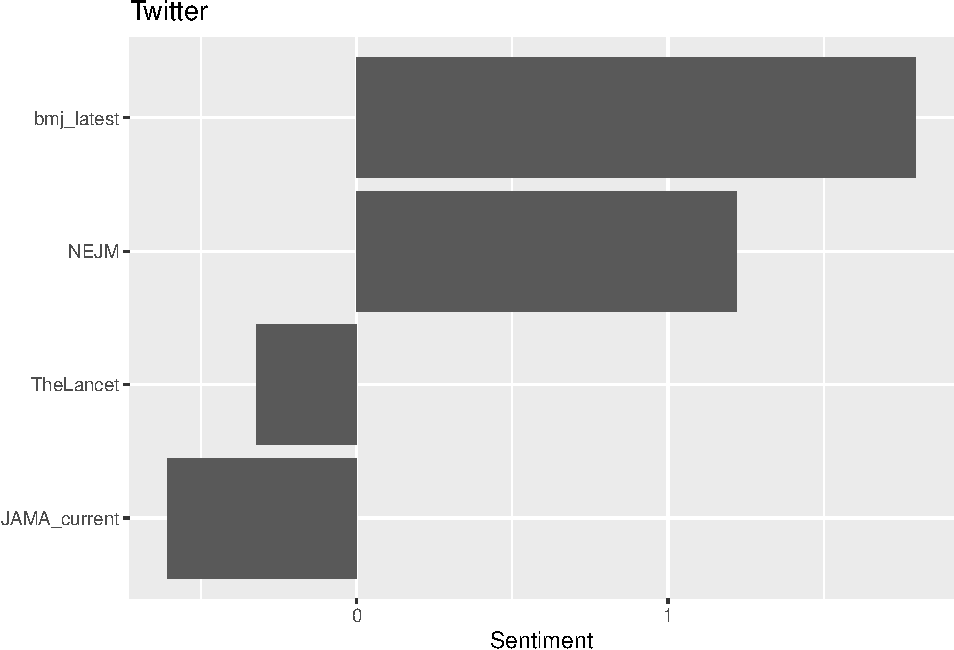
\includegraphics{nlp_tw_files/figure-latex/unnamed-chunk-4-1.pdf}

\end{document}
